\section*{Assignment 09: Scaling Strategy}
\addcontentsline{toc}{section}{Assignment 09: Scaling Strategy}

\subsection*{Phase one: proving product market fit}
The first phase happens in one city to keep coordination simple. I aim for sixty active students and twenty finished projects with satisfaction scores above four point five. These targets are based on the launch model in Assignment~02 and \citet{Choudary2016}'s idea of reaching a \textit{minimum viable critical mass} before expanding. Two main partners, ideally a municipal innovation unit and a trusted NGO network, give legitimacy. The team has a product lead, two engineers, a community manager, and part time mentor support. Weekly records every challenge in a shared knowledge base so that all improvements are backed by evidence.

\subsection*{Phase two: regional expansion}
Once the core loops work, the second phase grows across the region. Onboarding flows are turned into standard templates, and the API described in Assignment~06 helps partners connect without custom work. I set up a three tier partner program (community, certified, strategic) with rules for response time, satisfaction, and contribution to \textit{fairness metrics}. The goals increase to two hundred fifty active students, seventy five organisations, and a time to first value under twelve hours. These targets follow \citet{HagiuWright2013}'s focus on balancing growth and quality. A \textit{partner success pod} monitors retention and holds quarterly business reviews, using rituals from enterprise \textit{SaaS} while keeping the tone friendly.

\subsection*{Phase three: national network}
The final phase explores national or Nordic reach once unit economics stabilise. This step needs alliances with national agencies, expanded governance through an advisory board, and white label options for institutions that want their own branding. Success means five hundred projects per year, completion above ninety percent, and net revenue retention above one hundred ten percent. \citet{Srnicek2017} warns that scaling without legitimacy invites backlash, so transparency reports and the inclusion council stay central.

\subsection*{Risk mitigation and decision gates}
Two risks dominate scaling plans: \textit{churn} and \textit{quality drift}. To manage \textit{churn} I track retention in each segment, run exit interviews, and build loyalty through alumni storytelling events. To manage quality I set \textit{service level agreements} for response times, automate match quality checks, and call a community board if satisfaction stays below four point four for two months in a row. If that happens, onboarding of new partners stops until the board approves remediation steps. Figure~\ref{fig:scaling-dashboard} shows the dashboard that monitors these signals.

\begin{figure}[H]
  \centering
  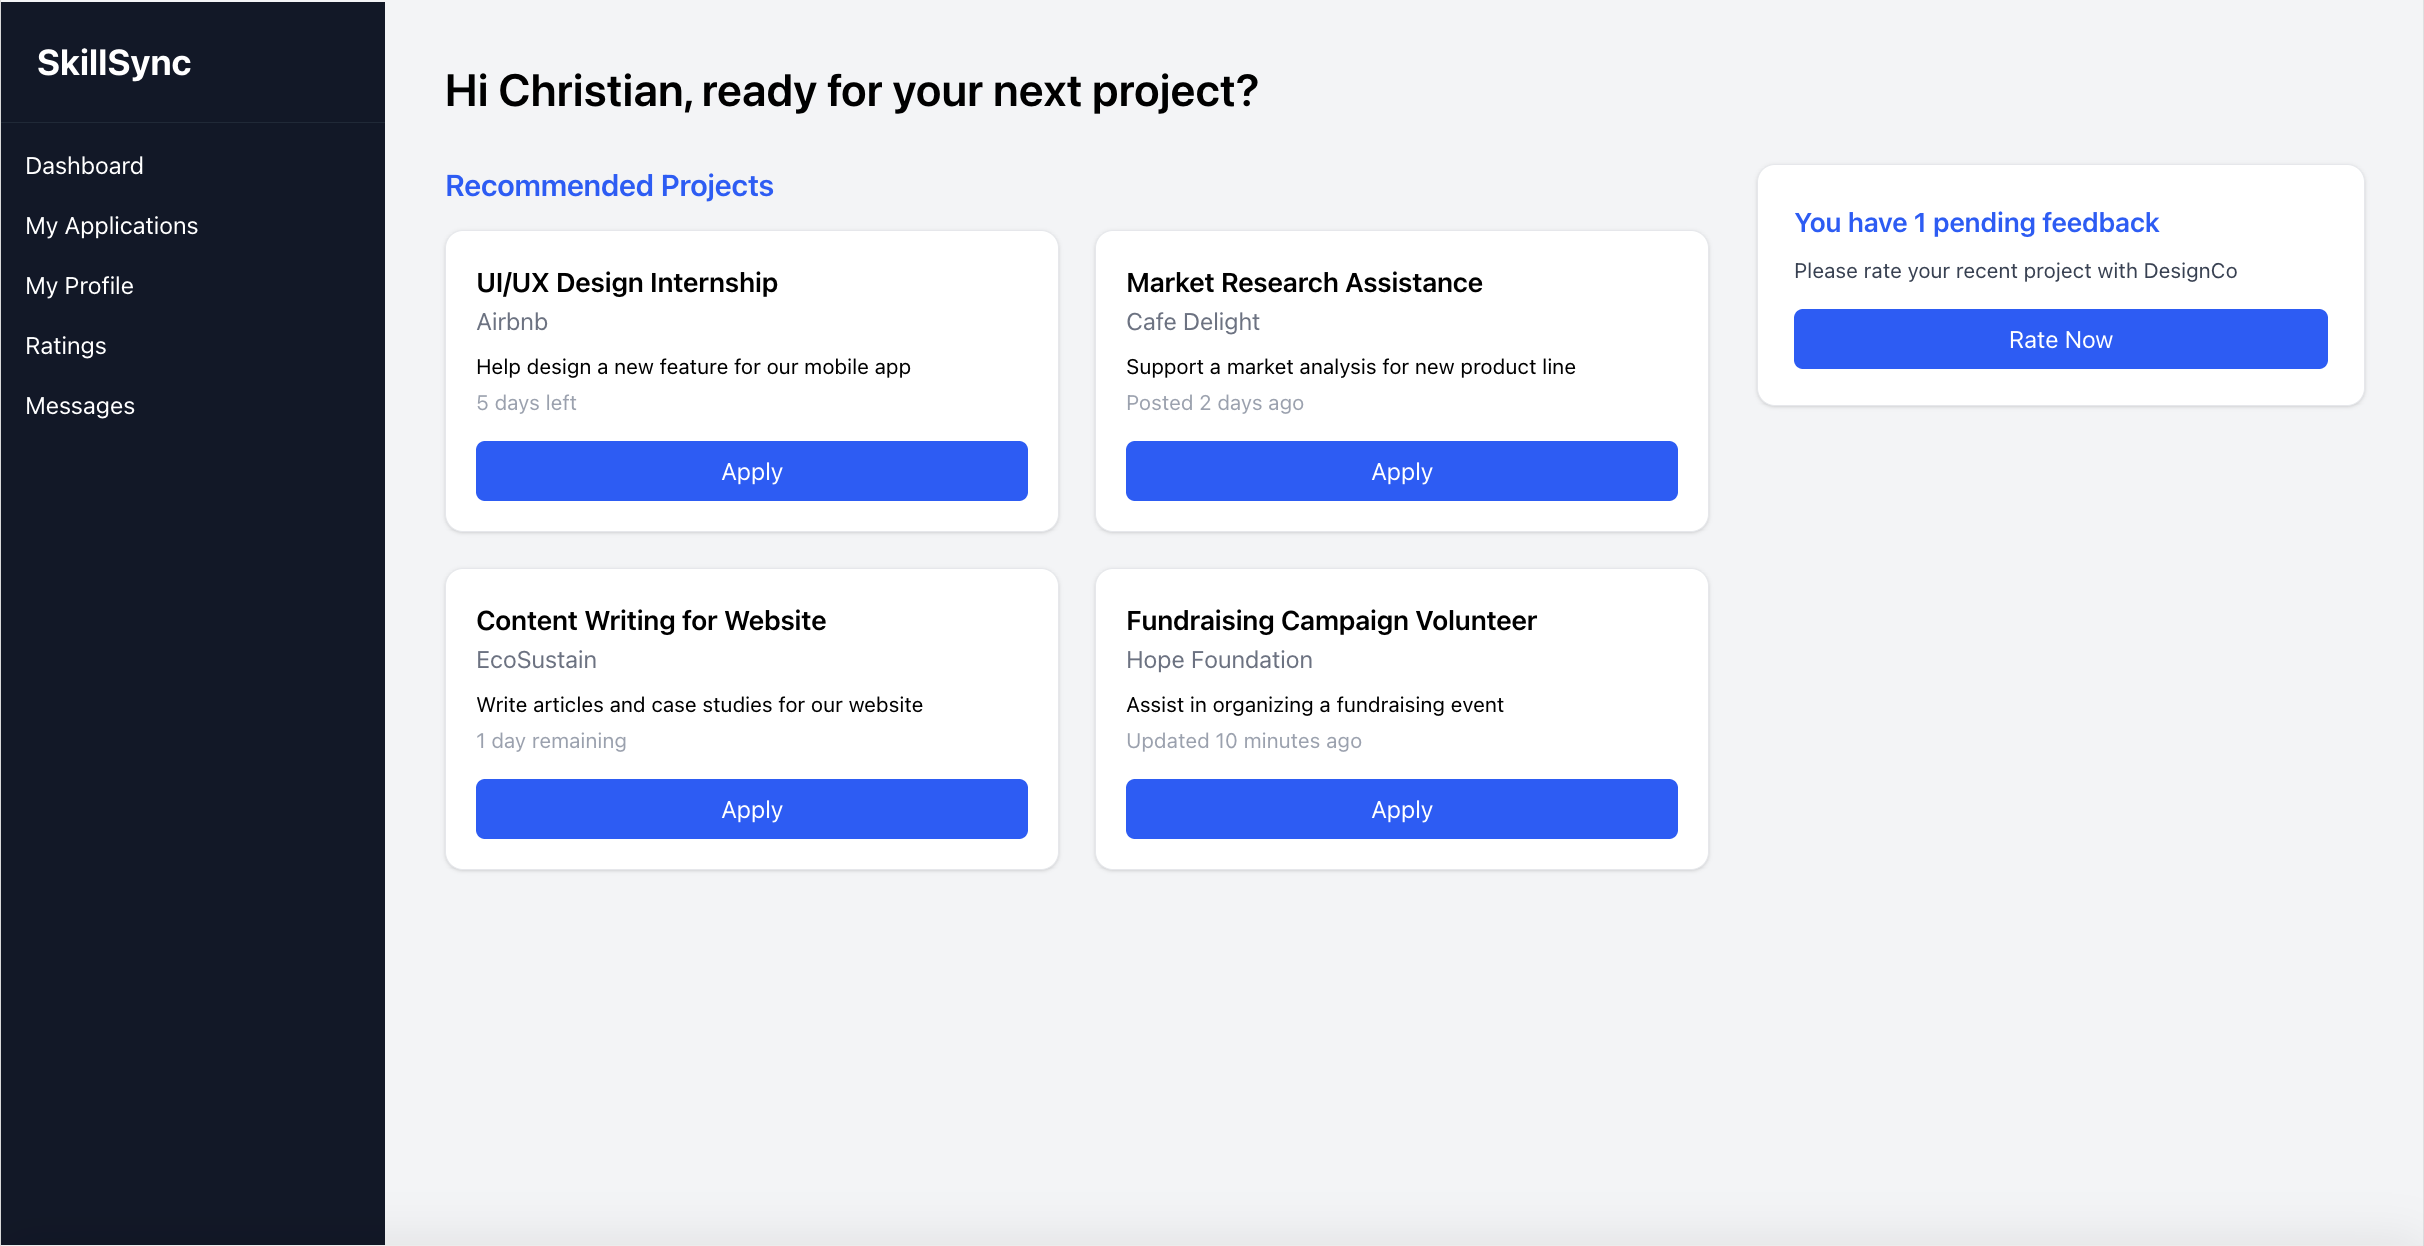
\includegraphics[width=0.75\linewidth]{figures/Student-Dashboard.png}
  \caption{Adoption dashboard mock up tracking activation against partner enablement.}
  \label{fig:scaling-dashboard}
\end{figure}

\subsection*{Scenario modelling}
To test resilience I built a Google Sheets simulation that tracks activation rate, moderation load, partner velocity, and revenue per project. The model estimates staff needs for every one thousand active users and includes a pause rule: if satisfaction stays below four point four for eight weeks, growth spending stops. I also made a downside case where retention drops five points. This reduces annual revenue by about nine million DKK and delays break even by twelve months. Because of this, the playbook includes a cost reduction plan that focuses on core trust features. These exercises follow \citet{Lecture12}'s advice to see scaling as a system design problem instead of a marketing stunt.
